\section{Training Data Samples}
\label{appdx:data_sample}
\subsection{Question Formation}

We use the term \textbf{declarations} to refer to the declaration copying task and \textbf{questions} refer to the question formation task. Here are two examples randomly taken from the training data: 

\begin{itemize}[itemsep=2pt,labelindent=0pt,topsep=0pt,parsep=0pt,partopsep=1pt, align=left, leftmargin=*]
    \item Declaration Example: \texttt{our zebra doesn't applaud the unicorn . decl	our zebra doesn't applaud the unicorn .}
    \item Question Example: \texttt{some unicorns do move . quest	do some unicorns move ?}
\end{itemize}

Both tasks begin with an input declarative sentence, followed by a task indicator token (\texttt{decl} or \texttt{quest}), and end with the output. During training, the entire sequence is used in the causal language modeling objective. The ID validation set and the OOD generalization set only contain question formation samples. In Figure \ref{fig:data_detail} (\textit{left}), we show a breakdown of two task types in QF training data. 


\subsection{Tense Inflection}
\begin{itemize}[itemsep=2pt,labelindent=0pt,topsep=0pt,parsep=0pt,partopsep=1pt, align=left, leftmargin=*]
   \item  Past Example: \texttt{our peacocks above our walruses amused your zebras . PAST	our peacocks above our walruses amused your zebras .}
    \item Present Example: \texttt{your unicorns that our xylophones comforted swam . PRESENT	your unicorns that our xylophones comfort swim .}
\end{itemize}
The tense inflection task is indicate by the \texttt{PRESENT} token. The secondary task only requires repeating the given sentence, which is always in the past tense, and the copying task is marked by the \texttt{PAST} token. In Appendix \ref{appdx:ti_secondary}, show that the past-tense copying task is not necessary.

\begin{figure}[t!]
    \centering
    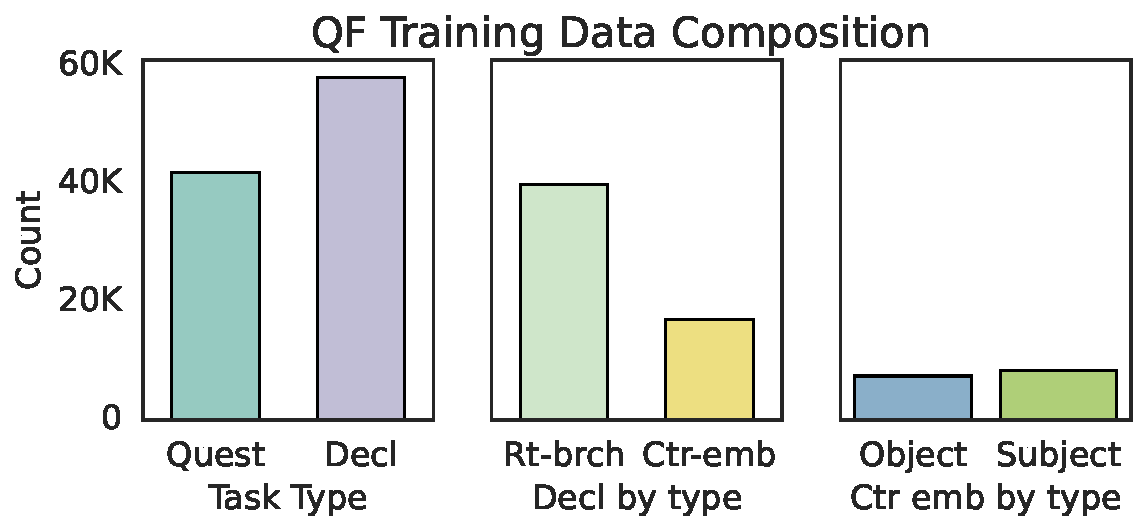
\includegraphics[width=0.49\linewidth]{figures/qf_data_composition.pdf}
    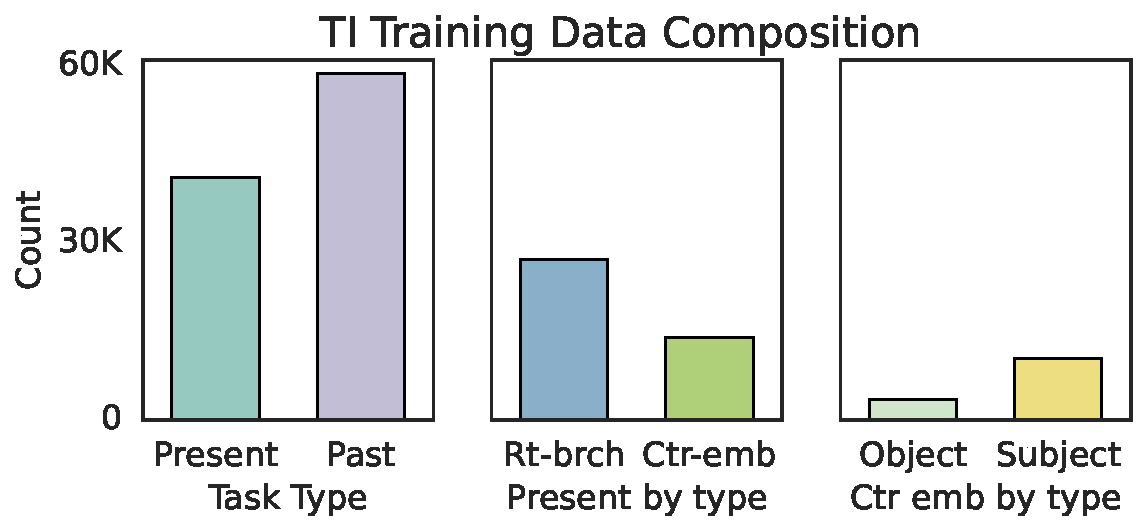
\includegraphics[width=0.49\linewidth]{figures/ti_data_composition.pdf}
    \caption{\textbf{Components of the original QF and TI training data.} 
    \textit{Left:} QF training data contains samples of two tasks types: question formation and declaration copying. We break down samples in the declaration copying task by branching type. We also breakdown center-embedded sentences based on whether the main subject serves the subject or object in the embedded clause.
    \textit{Right:} TI training data also contains samples of two task types: tense inflection and past tense copying. Similar to QF, we breakdown tense inflection samples by branching types, and breakdown center-embedded sentences in the tense inflection samples by subject/object type. 
    }
    \label{fig:data_detail}
\end{figure}

\section{Further Partitions on Center-Embedded Sentences}
\label{appdx:obj_sbj_ctr_breakdown}

\subsection{Two Subtypes of Center-Embedded Sentences}
In Section \ref{sec:data_complexity}, we showed that center-embedded sentences drive hierarchical generalization in both the QF and TI tasks. Here, we further partition center-embedded sentences based on the syntactic role of the \textit{main subject} (i.e., the subject of the main clause) within the modifying clause. Specifically, we classify them into two types:

\begin{enumerate}[itemsep=4pt,labelindent=2pt,topsep=0pt,parsep=0pt,partopsep=1pt,align=left,leftmargin=*]
    \item \textbf{Subject-type}: The main subject serves as the \textbf{subject} within the clause.

    Example: \textit{The keys that unlock the cabinet are on the table.}

    \item \textbf{Object-type}: The main subject serves as the \textbf{object} within the clause.
    
    Example:\textit{ The keys that the bear uses are on the table.}
\end{enumerate}

This partition is motivated by their distinct subject-verb dependency patterns. In subject-type sentences, both the main verb (from the main clause) and the embedded verb (from the relative clause) depend on the main subject. In contrast, object-type sentences exhibit a nested subject-verb structure. Our goal is to investigate whether differences in subject-verb dependency patterns influence the model’s preference for the hierarchical rule.



\begin{figure}[ht]
    \centering
    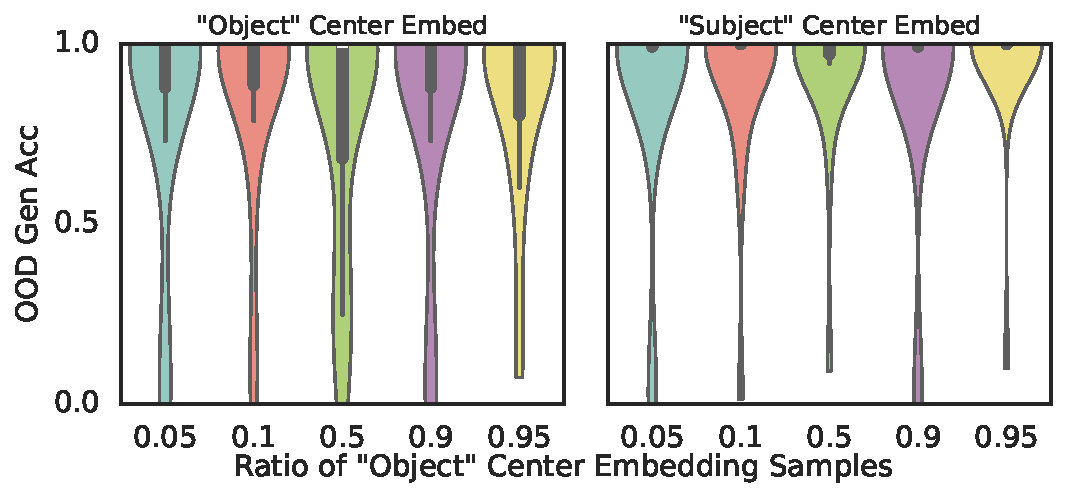
\includegraphics[width=0.6\linewidth]{figures/qf_rc_type.pdf}
    \caption{\textbf{Both subtypes of center-embedded sentences induce hierarchical generalization in QF.} We train models on datasets containing different ratios of object-type v.s. subject-type center-embedded sentences. We then evaluate on models on two OOD generalization set, one containing unambiguous object-type center-embedded sentences and the other unambiguous subject-type center-embedded sentences.}
    \label{fig:qf_rc_type}
\end{figure}

\subsection{QF Task Results}
The original QF training data contains roughly equal amount of two subtypes of center-embedded declarations, shown in Figure \ref{fig:data_detail} (\textit{left}). We investigate whether the two subtypes of center-embedded sentences differentially influence the model's preference for the hierarchical rule in the QF task. For all training data variants, we fix 50K question formation samples and 50K declaration copying samples, with the latter containing only center-embedded sentences but varying the ratio between the two subtypes. To analyze generalization behavior on a more granular level, we partition the generalization set (composed solely of center-embedded sentences) into the two subtypes as well. Models are trained on 30 random seeds, and results are shown in Figure \ref{fig:qf_rc_type}. Regardless of the data mix, the model consistently favors the hierarchical rule across both partitions of the generalization set. This suggests that, for question formation, both subtypes of center-embedded sentences equally contribute to the model's ability to identify the main auxiliary.



\begin{figure}[h]
    \centering
    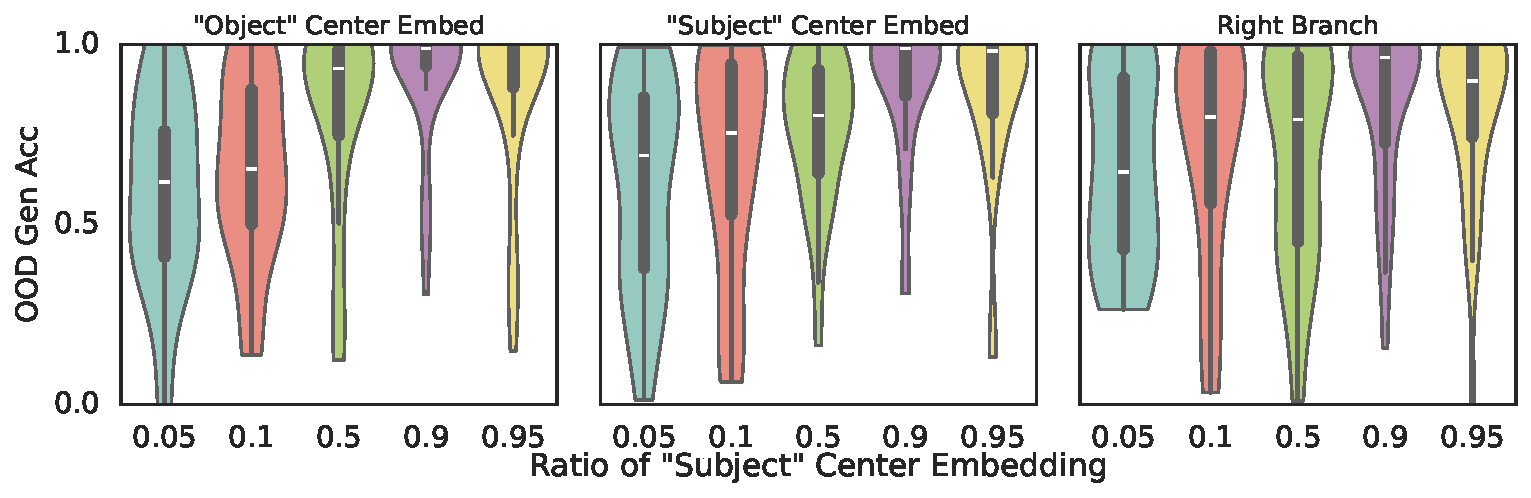
\includegraphics[width=0.9\linewidth]{figures/ti_rc_type.pdf}
    \caption{\textbf{Subject-type center-embedded sentences gives a stronger bias towards hierarchical generalization in TI.} We train models on datasets containing different ratios of object-type v.s. subject-type center-embedded sentences. We then evaluate on models on three OOD generalization set, one containing unambiguous object-type center-embedded sentences, one unambiguous subject-type center-embedded sentences, and one unambiguous right-branching sentences.}
    \label{fig:ti_rc_type}
\end{figure}

\subsection{TI Task Results} 
The original TI training data contains almost twice amount of subject-type center-embedded sentences than object-type ones, shown in Figure \ref{fig:data_detail} (\textit{left}).
We repeat a similar experiment for the TI task, fixing the total number of tense inflection samples to 100K. As shown in Section \ref{sec:ti_result}, models exhibit the strongest hierarchical generalization when trained on primarily center-embedded sentences. Therefore, in the following data variants, 99\% of the samples are center-embedded sentences, with the remaining 1\% being right-branching sentences. Within the center-embedded samples, we vary the ratio between the two subtypes. To evaluate generalization, we split the generalization set into three groups: the two subtypes of center-embedded sentences and right-branching sentences. Models trained on 30 random seeds show that, across all three generalization sets, accuracy is positively correlated with the proportion of subject-type center-embedded sentences (Figure \ref{fig:ti_rc_type}). However, even when models are trained predominantly on object-type center-embedded sentences (teal violins in Figure \ref{fig:ti_rc_type}), they still show a clear preference toward hierarchical generalization. Thus, while both subtypes drive hierarchical generalization in TI, subject-type center-embedded sentences have a stronger effect. 




\iffalse
% \subsection{Center Embedding is the Necessary Requirement}
\subsection{Relative Clauses Alone Cannot Induce Hierarchical Generalization}
\label{appdx:additionl_control}

\begin{figure}[t!]
    \centering
    \includegraphics[width=0.6\linewidth]{figures/no_curriculum_appdx.pdf}
    % 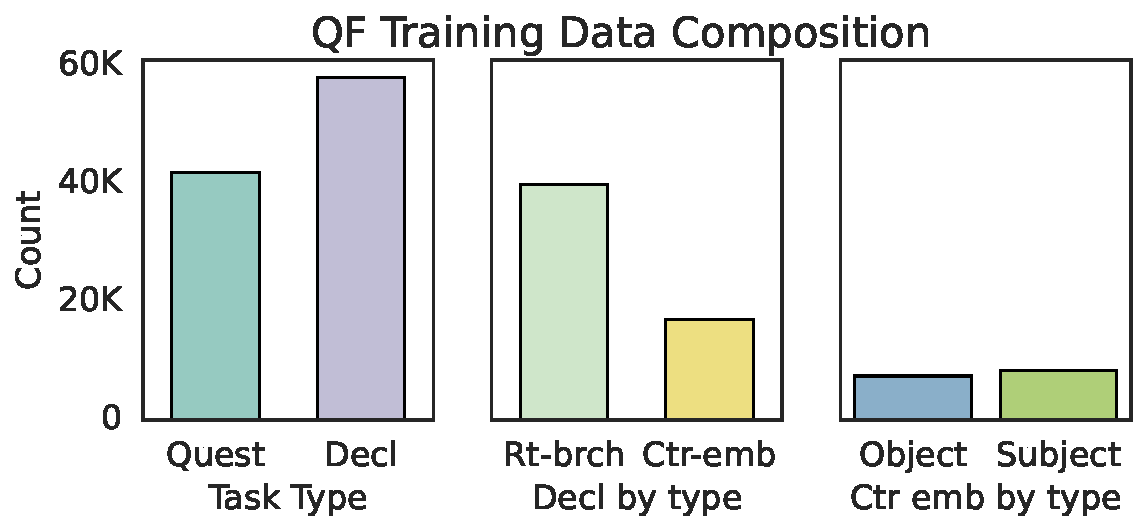
\includegraphics[width=0.4\linewidth]{figures/qf_data_composition.pdf}
    \caption{\textbf{Additional Experiment Control on QF Data} 
    \textit{Panel I$\&$II:} Partitioning declaration sentences by number of relative clauses, we see higher random variation among models trained on sentences with only one added clause, and similarly high random variation among models trained on a mix different clause counts.
    \textit{Panel III:} Sentences with one relative clause can be further partitioned based on whether the clause modifies the subject (center-embedded) or the object (right-branching). This additional evidence indicates that relative clause alone is not sufficient to induce hierarchical generalization.
    }
    \label{fig:grokking_selection_appdx}
   % \vspace{-5px}
\end{figure}


Center embedding imposes two constraints on syntax: (1) the sentence must include a relative clause, and (2) this clause must modify the subject. In contrast, right-branching sentences may or may not include a relative clause. The experiments from Section \ref{sec:qf_result} indicate that center-embedded sentences encourage the model to learn the hierarchical rule and generalize OOD. However, we have not ruled out the possibility that other data partitions could also induce hierarchical generalization. Specifically, the previous experiment did not control for the number of relative clauses.


In Figure \ref{fig:data_detail} \textit{left}, we show the breakdown of the question formation training data by different partitions. We now partition declarations based on the number of relative clauses they contain, creating three datasets, each with declarations limited to a specific number of relative clauses. Additionally, we conduct experiments on subsets where two of the three partitions are mixed, excluding the third. Results, shown in Figure \ref{fig:grokking_selection_appdx} (I and II), indicate that models trained on declarations without relative clauses fail to generalize hierarchically, while those trained on sentences with two relative clauses are more likely to succeed. This observation suggests an alternative hypothesis: that the number of relative clauses determines sentence complexity, with more complex sentences (i.e., those with additional relative clauses) encouraging the model to learn a tree-like syntactic representation.


However, experiments with declaration sentences containing one relative clause reveal that this alternative hypothesis is incorrect. 
With one relative clause, the clause either modifies the subject (center embedding) or the object (right branching). We retain samples with one relative clause in the declaration-copying task and further partition them by center embedding versus right branching. The distinct generalization behaviors, shown in Figure \ref{fig:grokking_selection_appdx} (III), indicate that when controlling for relative clause count, only center-embedded sentences induce the hierarchical rule. For sentences with two relative clauses, both the subject and object have clause modifiers, resulting in consistent center embedding. This explains why the number of relative clauses may initially appear to affect generalization behaviors.

\fi


\section{Varying Data Ratios for Question Formation}
\label{sec:simple_mixin}

\begin{wrapfigure}[17]{r}{0.4\textwidth}
    \vspace{-8px}
    \centering
    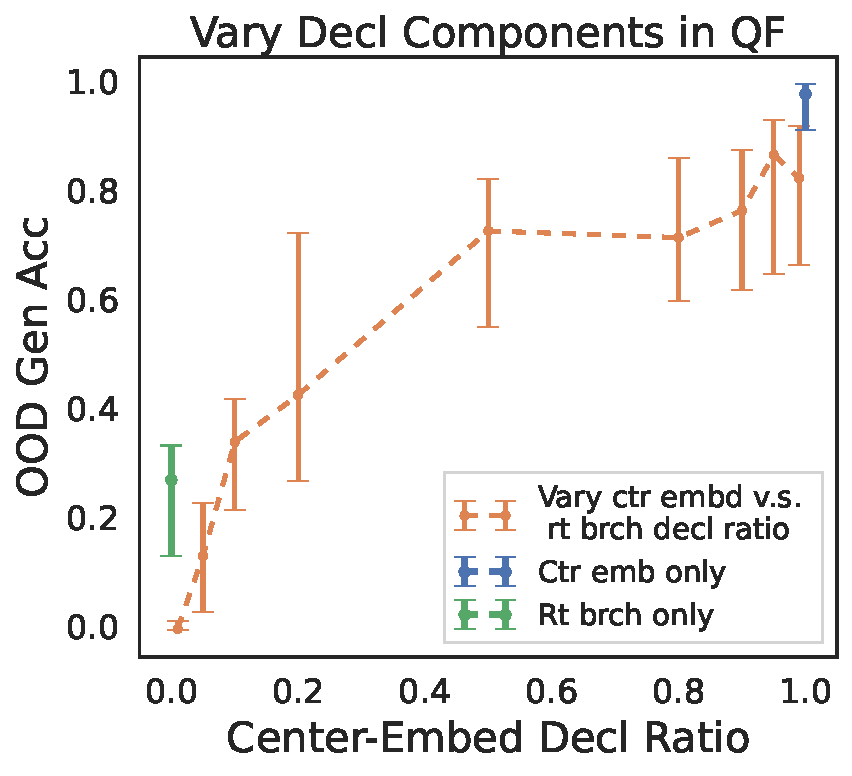
\includegraphics[width=0.9\linewidth]{figures/simplicity_contamination.pdf}
    \caption{Hierarchical generalization in QF is sensitive to compositions of declaration-copying samples.} 
    \label{fig:simplicity_contamination}
\end{wrapfigure}


\paragraph{Data composition details} We construct variations of the training data using the following procedure. Each new dataset contains 50K questions (reused from the original data) and 50K declarations, where we control the ratio between center-embedded and right-branching sentences. These datasets are used for the experiments in Section \ref{sec:intra_inter}. To generate additional declarations, we keep the distribution of the unique syntax structures in original dataset. Specifically, for each sentence in the original data, we extract the syntax tree using the CGF rules and resample words from the vocabulary to create new sentence samples. 

\paragraph{Sensitivity to data compositions}  We use the five datasets above to examine how different mix ratios affect a model's preference towards the hierarchical generalization. The median generalization accuracy, along with error bars representing the 35th and 65th percentiles, is shown in Figure \ref{fig:simplicity_contamination}. First, note that there is a sharp performance drop between the blue bar and the right-most orange bar. This sharp transition indicates that mixing in as little as 1\% of right-branching declarations significantly reduces the model's likelihood of generalizing hierarchically. Interestingly, when the dataset is predominantly right-branching declarations, models consistently achieve 0\% generalization accuracy, indicating a strong preference for the linear rule across all training runs. However, note that there is another sharp transition between the green bar and the left-most orange bar. This transition indicates that as soon as we remove the 1\% of center-embedded sentences, the model fails to learn either the linear rule or the hierarchical rule. As a result, the generalization accuracy is close to random guess ($\sim 25\%$). This transition is closely studied in Section \ref{sec:data_diveristy}, where we examine how data diversity leads to rule commitment. 


\section{Additional Results on Tense Inflection} 
\subsection{A Secondary Task is Not Necessary}
\label{appdx:ti_secondary}


\begin{wrapfigure}[14]{r}{0.4\textwidth}
    \vspace{-40px}
    \centering
    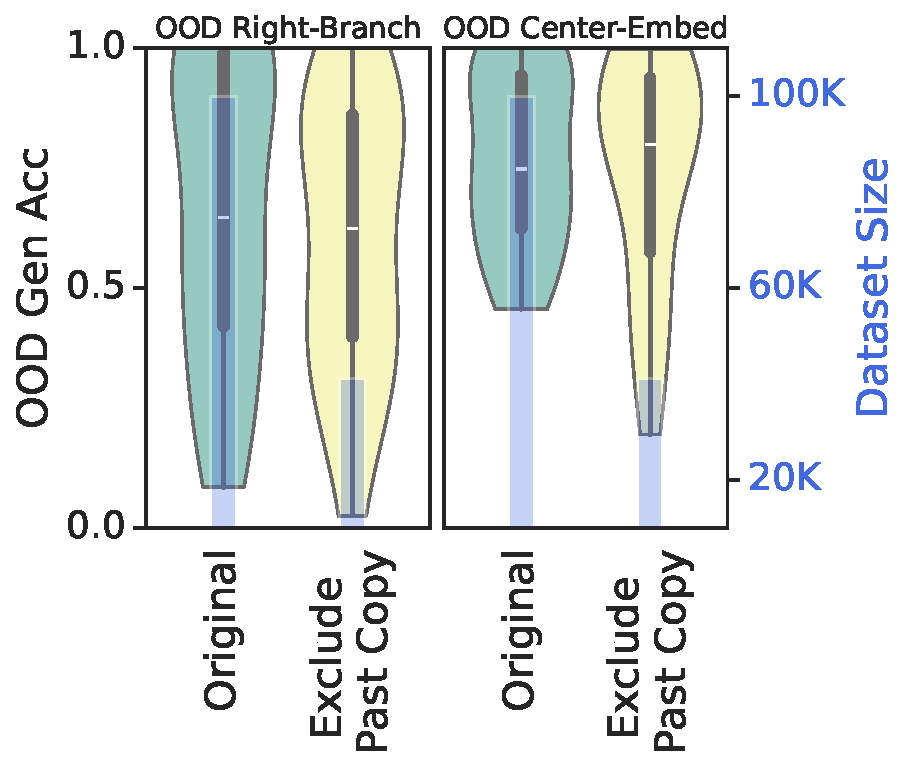
\includegraphics[width=1.0\linewidth]{figures/tense_inflection_violin.pdf}
    \caption{Past-copy task is not necessary to induce hierarchical generalization in TI.
    }
    \label{fig:tense_original_violin}
\end{wrapfigure}


In the original of TI training data \citep{McCoy2020-pj}, a secondary task is also included to mimic the question formation training data. In this secondary task, instead of transforming a sentence from the past tense to the present tense, the model simply needs to repeat it. For concrete examples, see Appendix \ref{appdx:data_sample}. Figure \ref{fig:data_detail} (\textit{right}) shows a breakdown of the two tasks in the original TI training data. In experiments conducted in Section \ref{sec:ti_task}, we have eliminated the used of this secondary task because center-embedded sentences can be included in the tense inflection training samples \textit{without} violating the ambiguity requirement. Here, we use the training data originally proposed by \citet{McCoy2020-pj} to confirm that the use of secondary task is indeed not necessary. Specifically, we remove all the past-tense-copying samples from the original training data and train models on the tense-inflection task only. We evaluate the model's generalization performance on two OOD set containing unambiguous right-branching and unambiguous center-embedded sentences, shown in Figure \ref{fig:tense_original_violin}. We can see that the model's OOD performances are the same with or without the secondary task. 


\subsection{Training Instability and Rule Commitment for TI}
\label{appdx:tense_tv}
\begin{figure}[t]
    \centering
    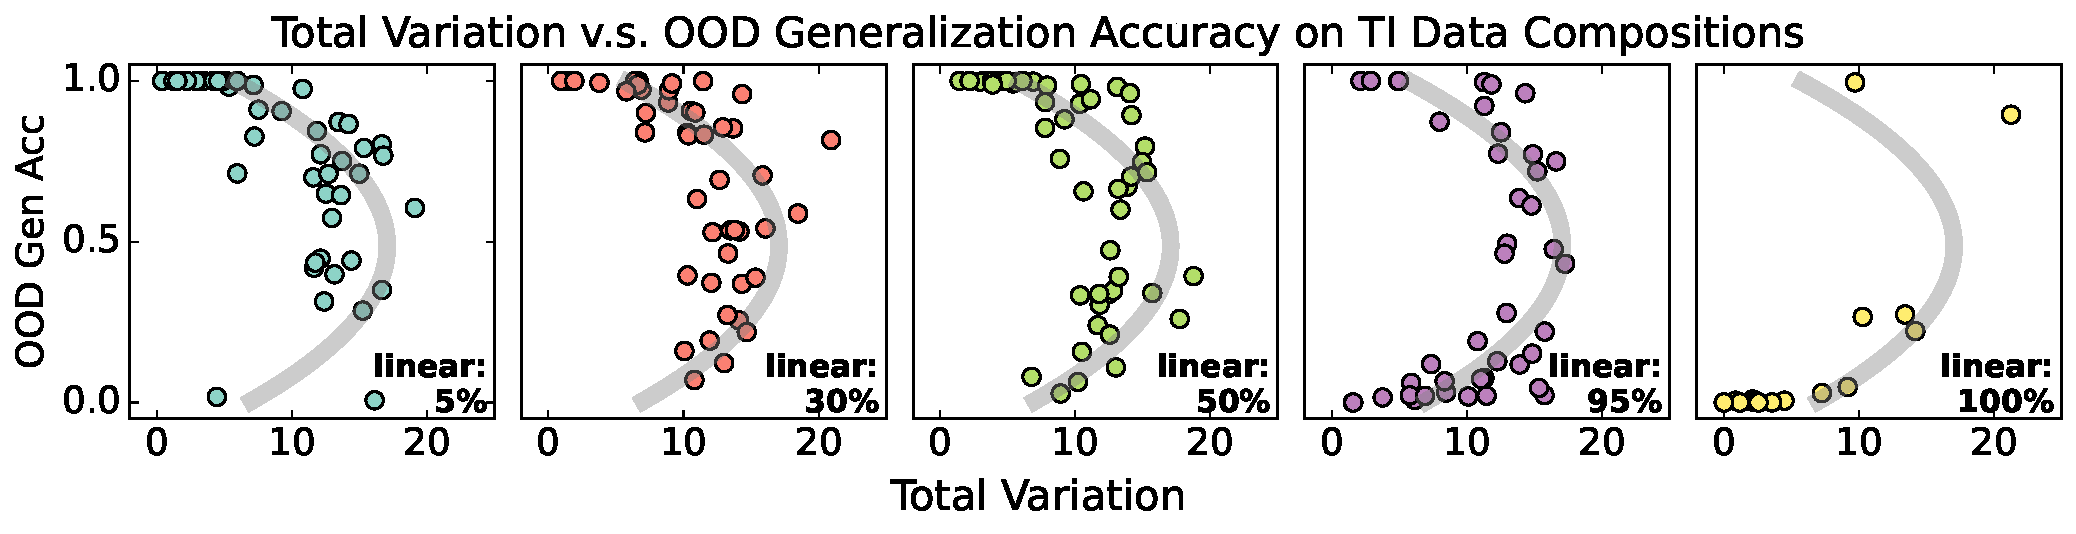
\includegraphics[width=1.0\linewidth]{figures/intra_inter_inconsistency_D101.pdf}
    \caption{\textbf{Total Variation v.s. final generalization accuracy for TI task.} Similar to Figure \ref{fig:intra_inter_variance}, we observe the same horseshoe shaped behavior between training stability and final generalization accuracy on right-branching sentences for the TI task.
    }
    \label{fig:intra_inter_variance_tense}
\end{figure}
We repeat the same total variation analysis in Section \ref{sec:stability} for the tense inflection task. We use the data mixes from Section \ref{sec:ti_result}. Specifically, we include only tense inflection samples and vary the ratio between linearity-inducing (i.e., right-branching) and hierarchy-inducing (i.e., center-embedded) sentences. In Section \ref{sec:ti_result}, we have already concluded that the hierarchical rule is \textit{always} preferred for center-embedded sentences regardless of data mixes. For this reason, we are interested in examining the rule preference and training stability for unambiguous right-branching sentences.
In Figure \ref{fig:intra_inter_variance_tense} we visualize the relationship between total variation and the final generalization accuracy on unambiguous right-branching sentences. The qualitative behavior is similar to what we have observed in QF (Section \ref{sec:intra_inter}).
% \begin{figure}[h]
%     \centering
%     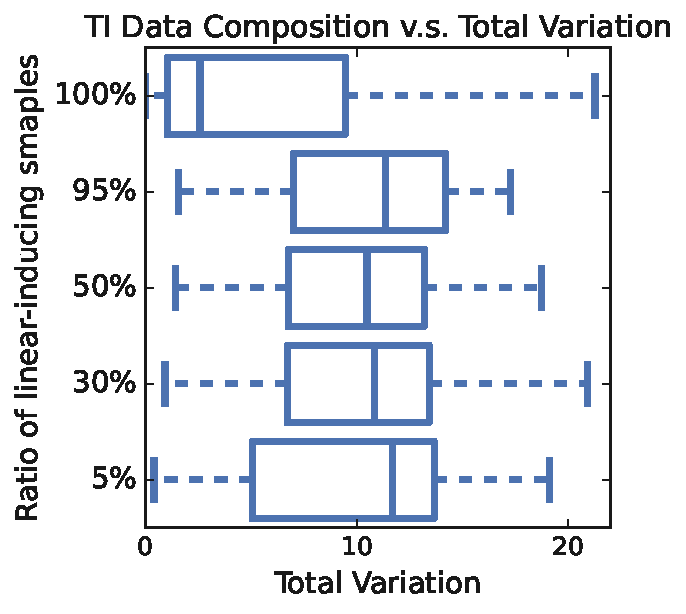
\includegraphics[width=0.3\linewidth]{figures/total_variation_box_ti.pdf}
%     \caption{Competition between subsets of data drives training inconsistency in tense inflection.}
%     \label{fig:data_drives_inconsistency_ti}
% \end{figure}

\section{Training Instability}
\label{appdx:training_instabilty}

\begin{figure}[h]
    \centering
    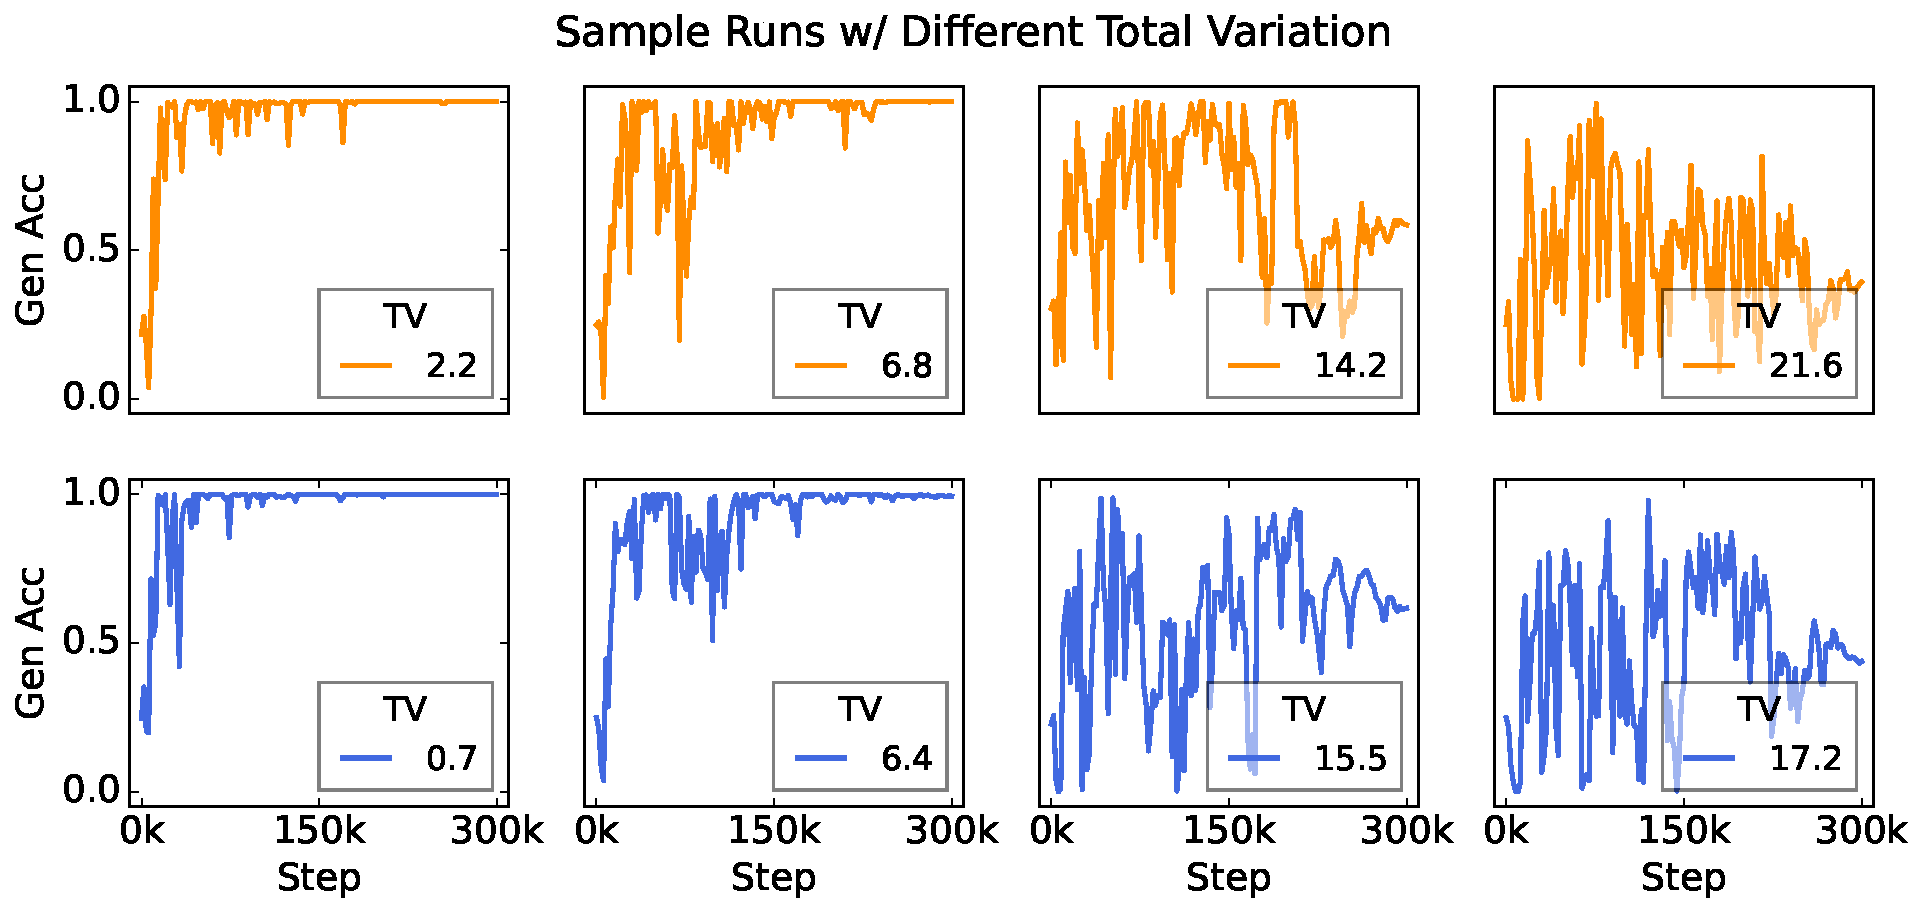
\includegraphics[width=0.66\linewidth]{figures/sample_runs.pdf}
    % \caption{Sample Runs with different total variation}
    \caption{\textbf{Each training run either stabilizes in a simple OOD generalization rule or oscillates in its OOD accuracy.} The OOD generalization behaviors can be either stable or unstable  when trained on different seeds. We use total variation to quantify the instability within one training run.}
    \label{fig:sample_runs}
\end{figure}

\begin{figure}[t]
    \centering
    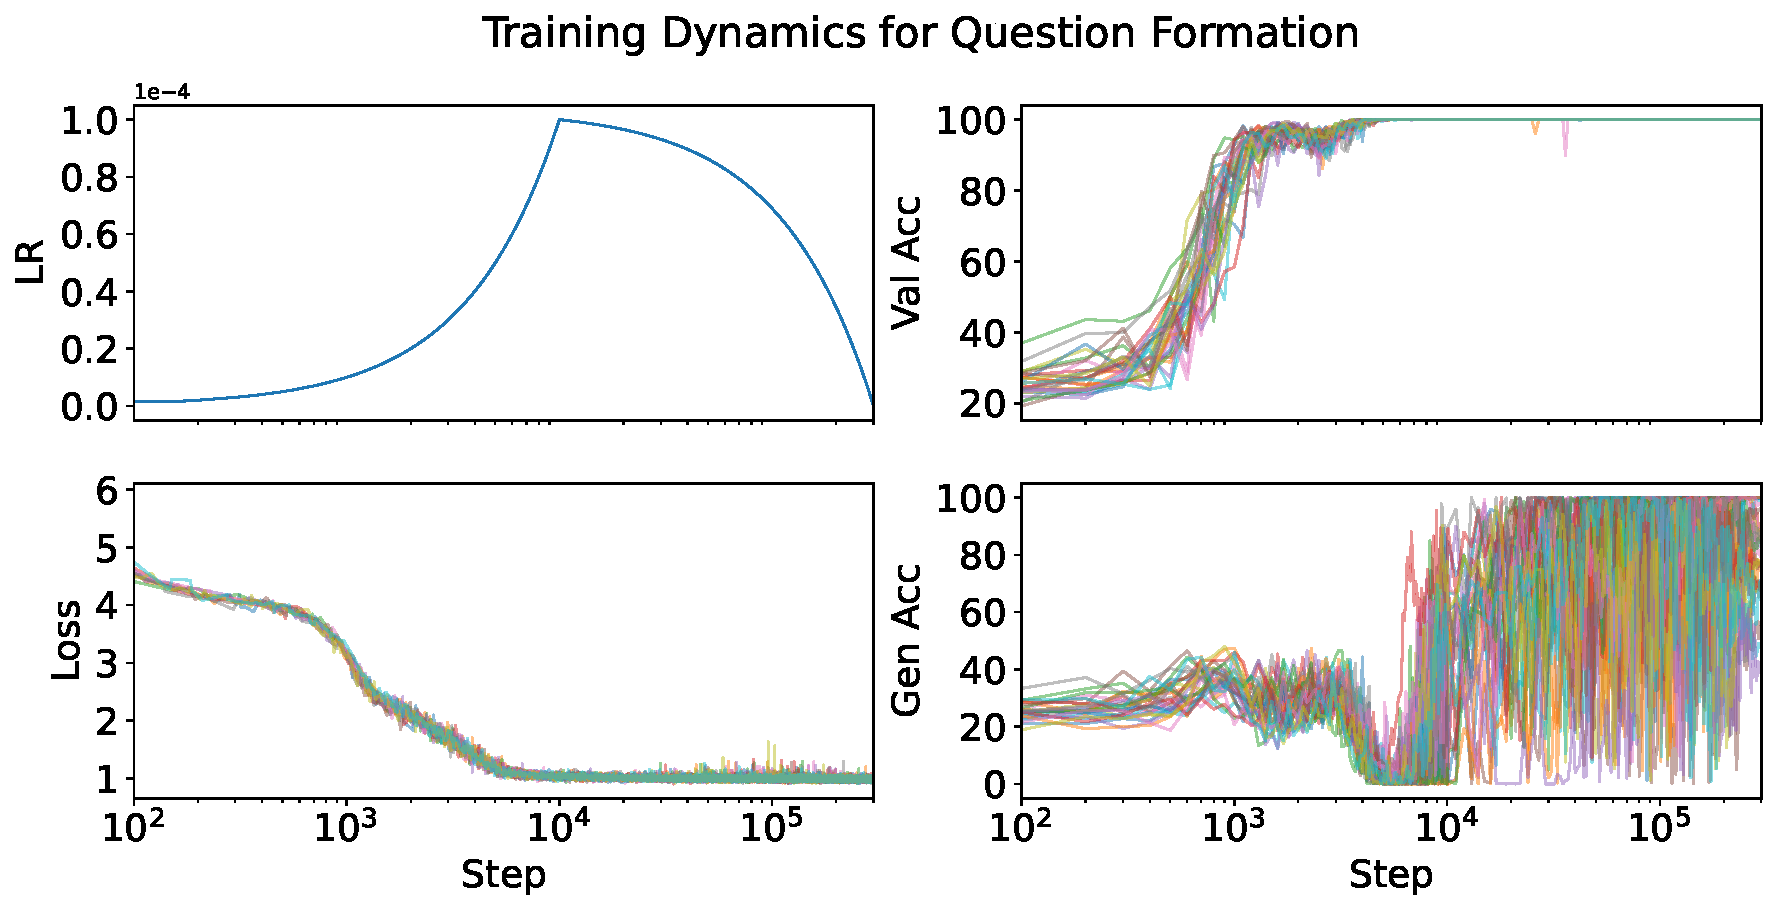
\includegraphics[width=.7\textwidth]{figures/warmup10k_lr1e-4_gradnorm1_trainig_dynamics.pdf}
    \caption{\textbf{Training dynamics on original QF data across 50 random seeds.} Training loss (\textit{lower left}) and in-distribution validation accuracy  (\textit{top right}) is stable during training and consistent across random seeds. In contrast, the model's performance on OOD generalization set (\textit{lower right}) is both unstable during training and inconsistent across seeds. The instability and inconsistency is most prominent during grokking (i.e., when training loss has converged). Even with a learning rate decay (\textit{top right}), the OOD behaviors for some seeds remain unstable throughout training.
    }
    \label{fig:grokking_inconsistency}
% \end{wrapfigure}
\end{figure}
In Figure \ref{fig:grokking_inconsistency}, we visualize the training dynamics for 30 independent runs when trained on the original QF data. Each run differs in both model initialization and data order. Notice that the training dynamics for runs exhibit grokking behaviors: OOD generalization is delayed when compared to training loss convergence and validation performance convergence. These runs share a similar progression in training loss, validation accuracy, and generalization accuracy up until moment when the training loss converges. 
Interestingly, after convergence on training loss, all runs reach $0\%$ on the generalization set, indicating that the model strictly prefers linear rules on OOD data. 
After that, models start to achieve non-trivial performance in generalization accuracy.
However, for many runs the generalization accuracy does not increase monotonically. Instead, we observe massive swings in generalization accuracy during this training period as well as large inconsistency across different seeds.
Overall, training is \textit{always} stable for ID data while the performance for OOD data is inconsistent across seeds. 
We visualize runs with different of total variation values in Figure \ref{fig:sample_runs}. 






\section{Data Diversity and Memorization Patterns}
\label{appdx:memorizaition}

\begin{figure}[h]
    \centering
    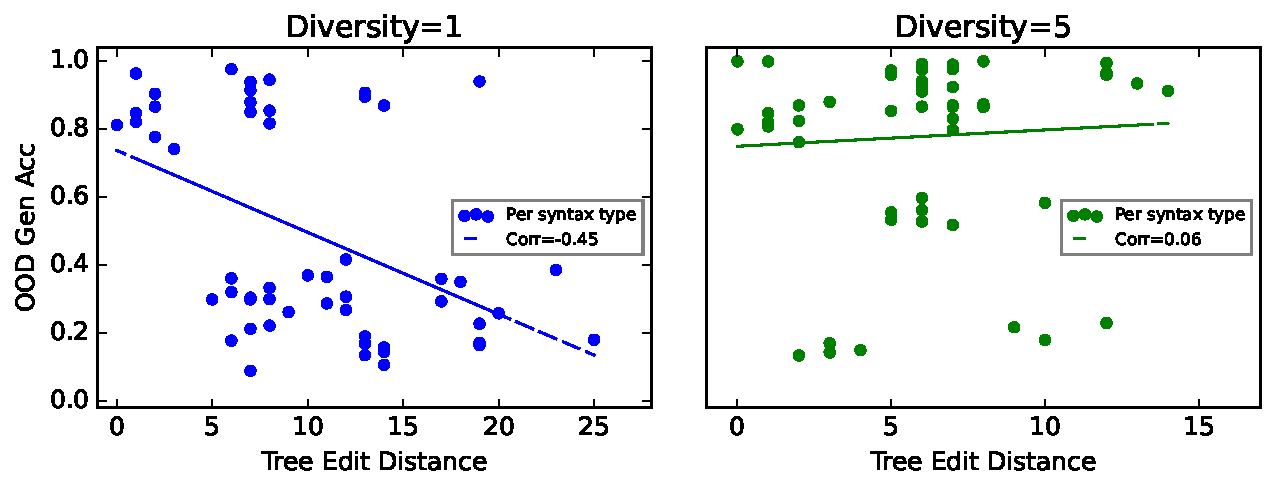
\includegraphics[width=0.8\linewidth]{figures/tree_edit_distance_performance.pdf}
    \caption{\textbf{OOD generalization vs. syntactic similarity to training data.} At low data diversity, model memorizes syntactic patterns and applies the hierarchical rule only on syntax structures similar to ones appeared in the training data. At high data diversity, model can extrapolates the hierarchical rule and can apply it even on unseen syntax structures that are dissimilar to training data.} 
    \label{fig:tree_edit_distance_performance}
\end{figure}

We investigate model behavior when trained on data with limited diversity. By analyzing a model's generalization accuracy across different syntactic types, we aim to distinguish patterns indicative of either memorization or generalization.

\paragraph{Measuring data similarity} Building on the diversity measure from Section \ref{sec:data_diveristy}, we now use Tree-Edit Distance (TED) as a measure of sentence similarity. As before, we first construct syntax trees using CFG rules, then calculate TED using the Zhang-Shasha Tree-Edit Distance algorithm \citep{Zhang1989-ma}. We define TED=0 for sentences that share the same syntax structure but differ only in vocabulary. This similarity measure allows us to quantify, for each sample in the OOD generalization set, the closest matching sentence type in the training data. In the memorization regime, where the model encounters only a few syntax types, we suspect it cannot extrapolate rules to syntactically distinct OOD sentences. In contrast, with a more diverse syntax exposure, rule extrapolation may enable the model to apply rules even to OOD sentence types.


\paragraph{Experiment} To verify our intuition about memorization and generalization, we train models on two variations of the QF data. In the first variation, the declaration-copying task has data diversity set to 1, meaning only one syntax type appears, and we specifically choose one with center embedding. In the second variation, the declaration-copying task has diversity set to 5, with all 5 types containing center embeddings. For both datasets, the question-formation task remains unchanged, consisting solely of right-branching sentences. 
For the diversity=1 dataset, we calculate TED for each unique syntax type in the OOD set against the single syntax type in the declaration-copying task. For the diversity=5 dataset, we compute TED between each OOD sample and the five syntax types in the declaration-copying task, taking the minimum. This TED score provides a measure of similarity between the OOD samples and those encountered during training.
Our goal is to determine, based on training with these datasets, which OOD syntax types the model applies the hierarchical rule to. 



\paragraph{Result} In Figure \ref{fig:tree_edit_distance_performance}, we visualize the final generalization accuracy for each OOD syntax type against its TED relative to the training data. When trained on low-diversity data (Figure \ref{fig:tree_edit_distance_performance}, \textit{left}), generalization accuracy is negatively correlated with TED. For syntax types seen in the declaration-copying task (TED=0) and those similar to it, the model applies the hierarchical rule. However, for syntax types with high TED, the model’s behavior is random (25\%), indicating failure to follow any rule. As data diversity increases slightly (Figure \ref{fig:tree_edit_distance_performance}, \textit{right}), generalization accuracy no longer correlates with TED, suggesting that once the model begins to extrapolate the hierarchical rule, it can apply this rule to a wider range of OOD syntax types.



\iffalse
\section{Additional Plots For Section \ref{sec:stability}}
\todo{Update plot and write some explanation}
\begin{figure}
    \centering
    \includegraphics[width=0.9\linewidth]{figures/intra_inter_inconsistency_3.png}
    \linebreak
    \includegraphics[width=0.5\linewidth]{figures/intra_inter_inconsistency_1.png}
    \linebreak
    \includegraphics[width=0.7\linewidth]{figures/intra_inter_inconsistency_2.png}
   
    \caption{\textbf{Three Different Inconsistency Behaviors.} \textit{Top:} Hierarchical Rule is Preferred. \textit{Middle:} Linear Rule is Preferred. \textit{Bottom:} No consistent rule is learned. }
    \label{fig:intra_inter_inconsistency_original}
\end{figure}



\begin{figure}[h]
    \centering
    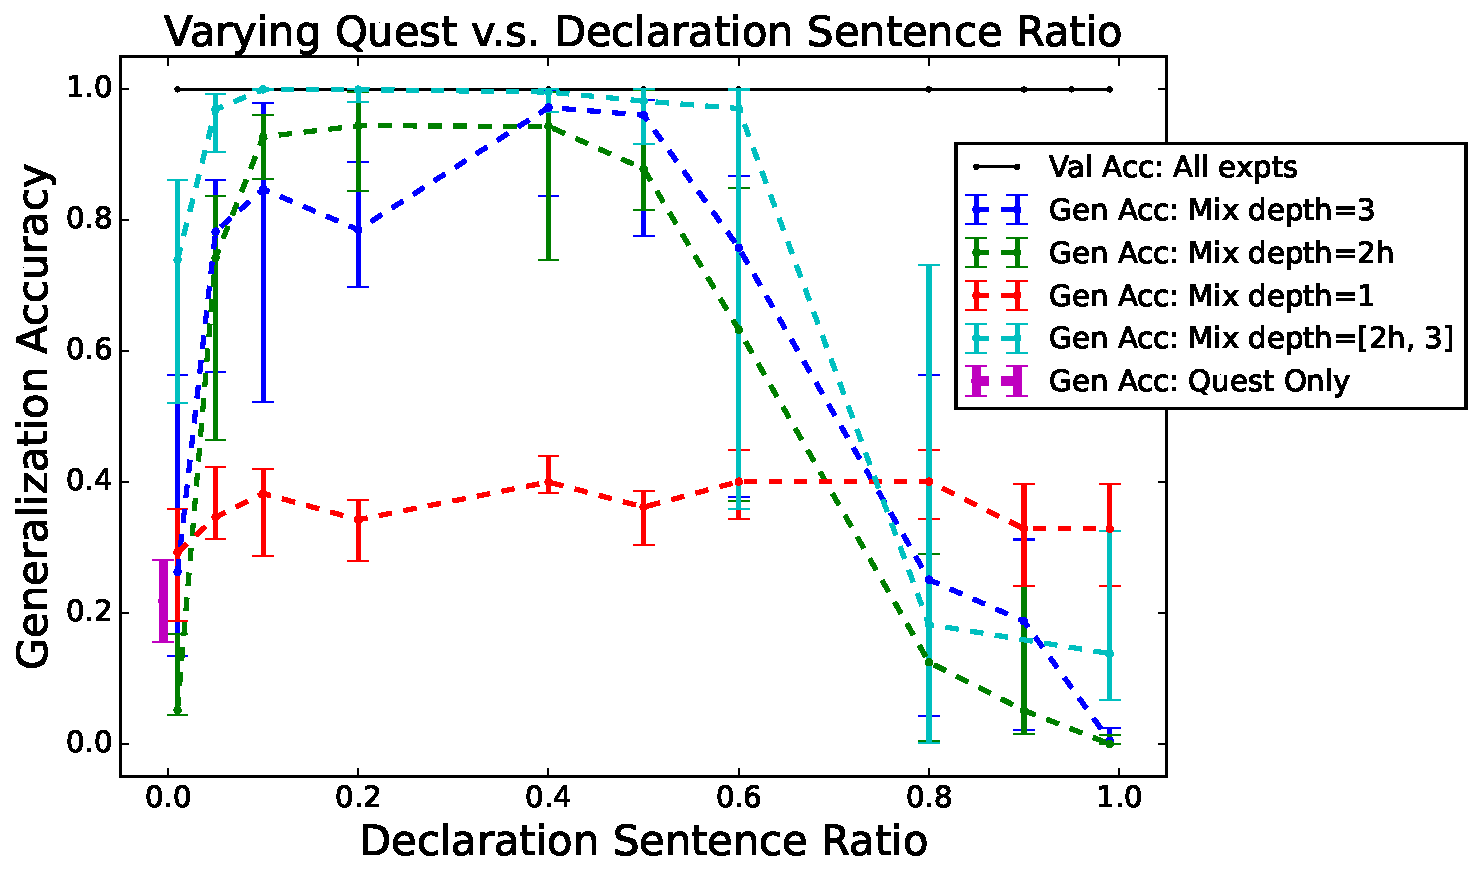
\includegraphics[width=1.0\textwidth]{figures/quest_decl_ratio.pdf}
    \caption{\textbf{Quest and Decl Ratio} Data size is standardized to 100k. We vary question and declaration ratios. For declarations, we also vary the the sentence typs mixes. \ns{for iclr we want to figure out why depth 1 doesn't teach a consistent rule at all. Also I don't understand how this plot would suggest depth one teaches no rule while it seems to give consistent linear rules based on figure 4} }
    \label{fig:quest_decl_ratio}
\end{figure}



\fi